\documentclass[12pt,a4paper]{article}
\usepackage[utf8]{inputenc}
\usepackage[T1]{fontenc}
\usepackage{geometry}
\usepackage{graphicx}
\usepackage{xcolor}
\usepackage{titlesec}
\usepackage{fancyhdr}
\usepackage{listings}
\usepackage{amsmath}
\usepackage{amsfonts}
\usepackage{hyperref}
\usepackage{booktabs}
\usepackage{array}
\usepackage{enumitem}
\usepackage{float}
\usepackage{caption}
\usepackage{subcaption}
\usepackage{tikz}
\usepackage{tcolorbox}
\usepackage{setspace}

% Set up geometry
\geometry{
    top=2.5cm,
    bottom=2.5cm,
    left=2.5cm,
    right=2.5cm
}

% Define colors matching the provided image
\definecolor{cse404green}{RGB}{76, 175, 80}
\definecolor{orangetitle}{RGB}{255, 152, 0}
\definecolor{bluepurple}{RGB}{121, 85, 178}
\definecolor{tealblue}{RGB}{69, 90, 100}
\definecolor{lightgray}{RGB}{245, 245, 245}

% Custom title formatting
\titleformat{\section}
{\normalfont\Large\bfseries\color{bluepurple}}
{\thesection}{1em}{}

\titleformat{\subsection}
{\normalfont\large\bfseries\color{tealblue}}
{\thesubsection}{1em}{}

% Set up hyperref
\hypersetup{
    colorlinks=true,
    linkcolor=bluepurple,
    filecolor=magenta,
    urlcolor=tealblue,
    pdftitle={Call of Duty Weapon Knowledgebase Report},
    pdfauthor={Sharif Md. Yousuf}
}

% Custom code listing style
\lstset{
    backgroundcolor=\color{lightgray},
    basicstyle=\ttfamily\small,
    breaklines=true,
    frame=single,
    numbers=left,
    numberstyle=\tiny\color{gray},
    keywordstyle=\color{blue},
    commentstyle=\color{green!60!black},
    stringstyle=\color{red}
}

\begin{document}

% Front page design matching the provided image
\begin{titlepage}
    \centering

    % CSE 404 Header Box
    \vspace*{2cm}
    {\Huge\bfseries\color{white}
        \colorbox{cse404green}{\makebox[8cm][c]{CSE 404}}
    }

    \vspace{1cm}

    % Main Title
    {\Huge\bfseries\color{orangetitle}
        Artificial Intelligence and\\
        Expert Systems Lab
    }

    \vspace{2cm}

    % Technical Report Title
    {\Large\bfseries\color{tealblue}
        Technical Report on \\ Call of Duty Weapon Knowledgebase
    }

    \vspace{0.5cm}

    {\large\color{bluepurple}
        Submission Date: 2/8/2025
    }

    \vspace{3cm}

    % Two column layout for submission info
    \begin{minipage}[t]{0.45\textwidth}
        \centering
        {\Large\bfseries\color{white}
            \colorbox{bluepurple}{\makebox[5cm][c]{Submitted by}}
        }

        \vspace{0.5cm}

        {\large\bfseries Name: Sharif Md. Yousuf}

        \vspace{0.3cm}

        {\large Registration ID:\@ 22101128}

        \vspace{0.3cm}

        {\large Section: C-2}

        \vspace{0.3cm}

        {\large Semester: 4-1}

        \vspace{0.3cm}

        {\large Session: Spring 2025}
    \end{minipage}
    \hfill
    \begin{minipage}[t]{0.45\textwidth}
        \centering
        {\Large\bfseries\color{white}
            \colorbox{tealblue}{\makebox[5cm][c]{Submitted to}}
        }

        \vspace{0.5cm}

        {\large\bfseries Bidita Sarkar Diba}

        \vspace{0.3cm}

        {\large Lecturer}

        \vspace{0.3cm}

        {\large Department of Computer}

        \vspace{0.3cm}

        {\large Science \& Engineering}

        \vspace{0.3cm}

        {\large University of Asia Pacific}
    \end{minipage}

    \vfill

\end{titlepage}

% Remove page numbering for title page and table of contents
\pagenumbering{gobble}

% Table of Contents
\tableofcontents
\newpage

% Start page numbering from here
\pagenumbering{arabic}
\setcounter{page}{1}

% Main Content
\section{Problem Title}

\textbf{Call of Duty Weapon Knowledgebase: Building a Smart Gaming Arsenal System with Prolog}

As a gamer, Call of Duty has always allowed me to take inspiration from the
complex weapon systems that exist in each of its different games. Having 121
weapons from 18 games, together with numerous attachments and complex unlock
chains, I kept wondering: "What is the best approach to unlock this weapon?"
and "Which attachments do best go with each other?"

This project is the answer for such questions. It creates a Prolog
knowledge-base for the Call of Duty weapon ecosystem. It does not only store
information in a mere database, but it is able to trace unlock paths, suggest
optimal builds, and analyze relationships among weapons spanning two decades of
gaming history.

\section{Problem Description}

As an experienced Call of Duty player, I often found the subversion of my own
patience with the vexing weapon systems across diverse titles-being achieving
the ad hoc remembrance of attachment compatibility with various guns, the
adornment of the best unlock path for activeness, or performance optimizations
in numerous concrete playstyles. With 121 weapons spread over 18 different
titles, innumerable attachments, and multi-level progressions, my research time
very often exceeded the time I actually spent on building and playing. Being
born out of frustration: build a smart Prolog knowledge-based entity that could
answer instant queries of the sort "Fastest way to unlock XM4?" or "Attachments
that make MP5 better for stealth gameplay?" Now, instead of manually digging
through wikis and forums, one can ask that particular intelligent ABS that
comprehends interrelations of weapons and attachments, as well as game
mechanics, across two decades of Call of Duty history. The harder aspect was
not the storage of data, but rather ensuring that the program was able to sift
through huge branching unlock chains, optimally recommend builds, and even take
into account the fact that weapon systems have evolved significantly from the
simple mechanics of Call of Duty 1 to the deepest-level systems in modern
titles.

\section{Tools and Languages Used}

I selected SWI-Prolog 9.0+ as my chief development framework considering that
it can beautifully deal with complex logical relationships-being gallant for
models of weapon unlock chains and weapon attachment compatibility, which
constitutes a familiar working system in gaming. Visual Studio Code became my
editor since it included excellent Prolog extensions and stopped syntax errors
even before considering any code run. It also had integrated Git features that
helped me stay abreast of many iterations I went through. LaTeX took charge of
the report layout (I admit that curve is almost vertical at first), but once I
adapted to it, it was a morale boost having it keep the whole citations and
code formatting half of a headache away in contrast to working within Word. I
then used Mermaid diagrams for visualizing the complex weapon progression
trees-so instead of explaining unlock chains via long convoluted paragraphs, I
could just plainly and completely present how the M4A1 unlocks the ACR, which
in turn unlocks the MK14. Custom test suites were being developed throughout
the development, injecting over 50 test cases to affirm correctness, vital to
discovering edge cases in my recursive algorithms.

\section{Diagram/Figure}

The knowledge base architecture is built on a layering approach with separation
of concerns, as shown in Figure 1. The system consists of several
interconnected layers that handle the various facets of the weapon ecosystem.

\begin{figure}[H]
    \centering
    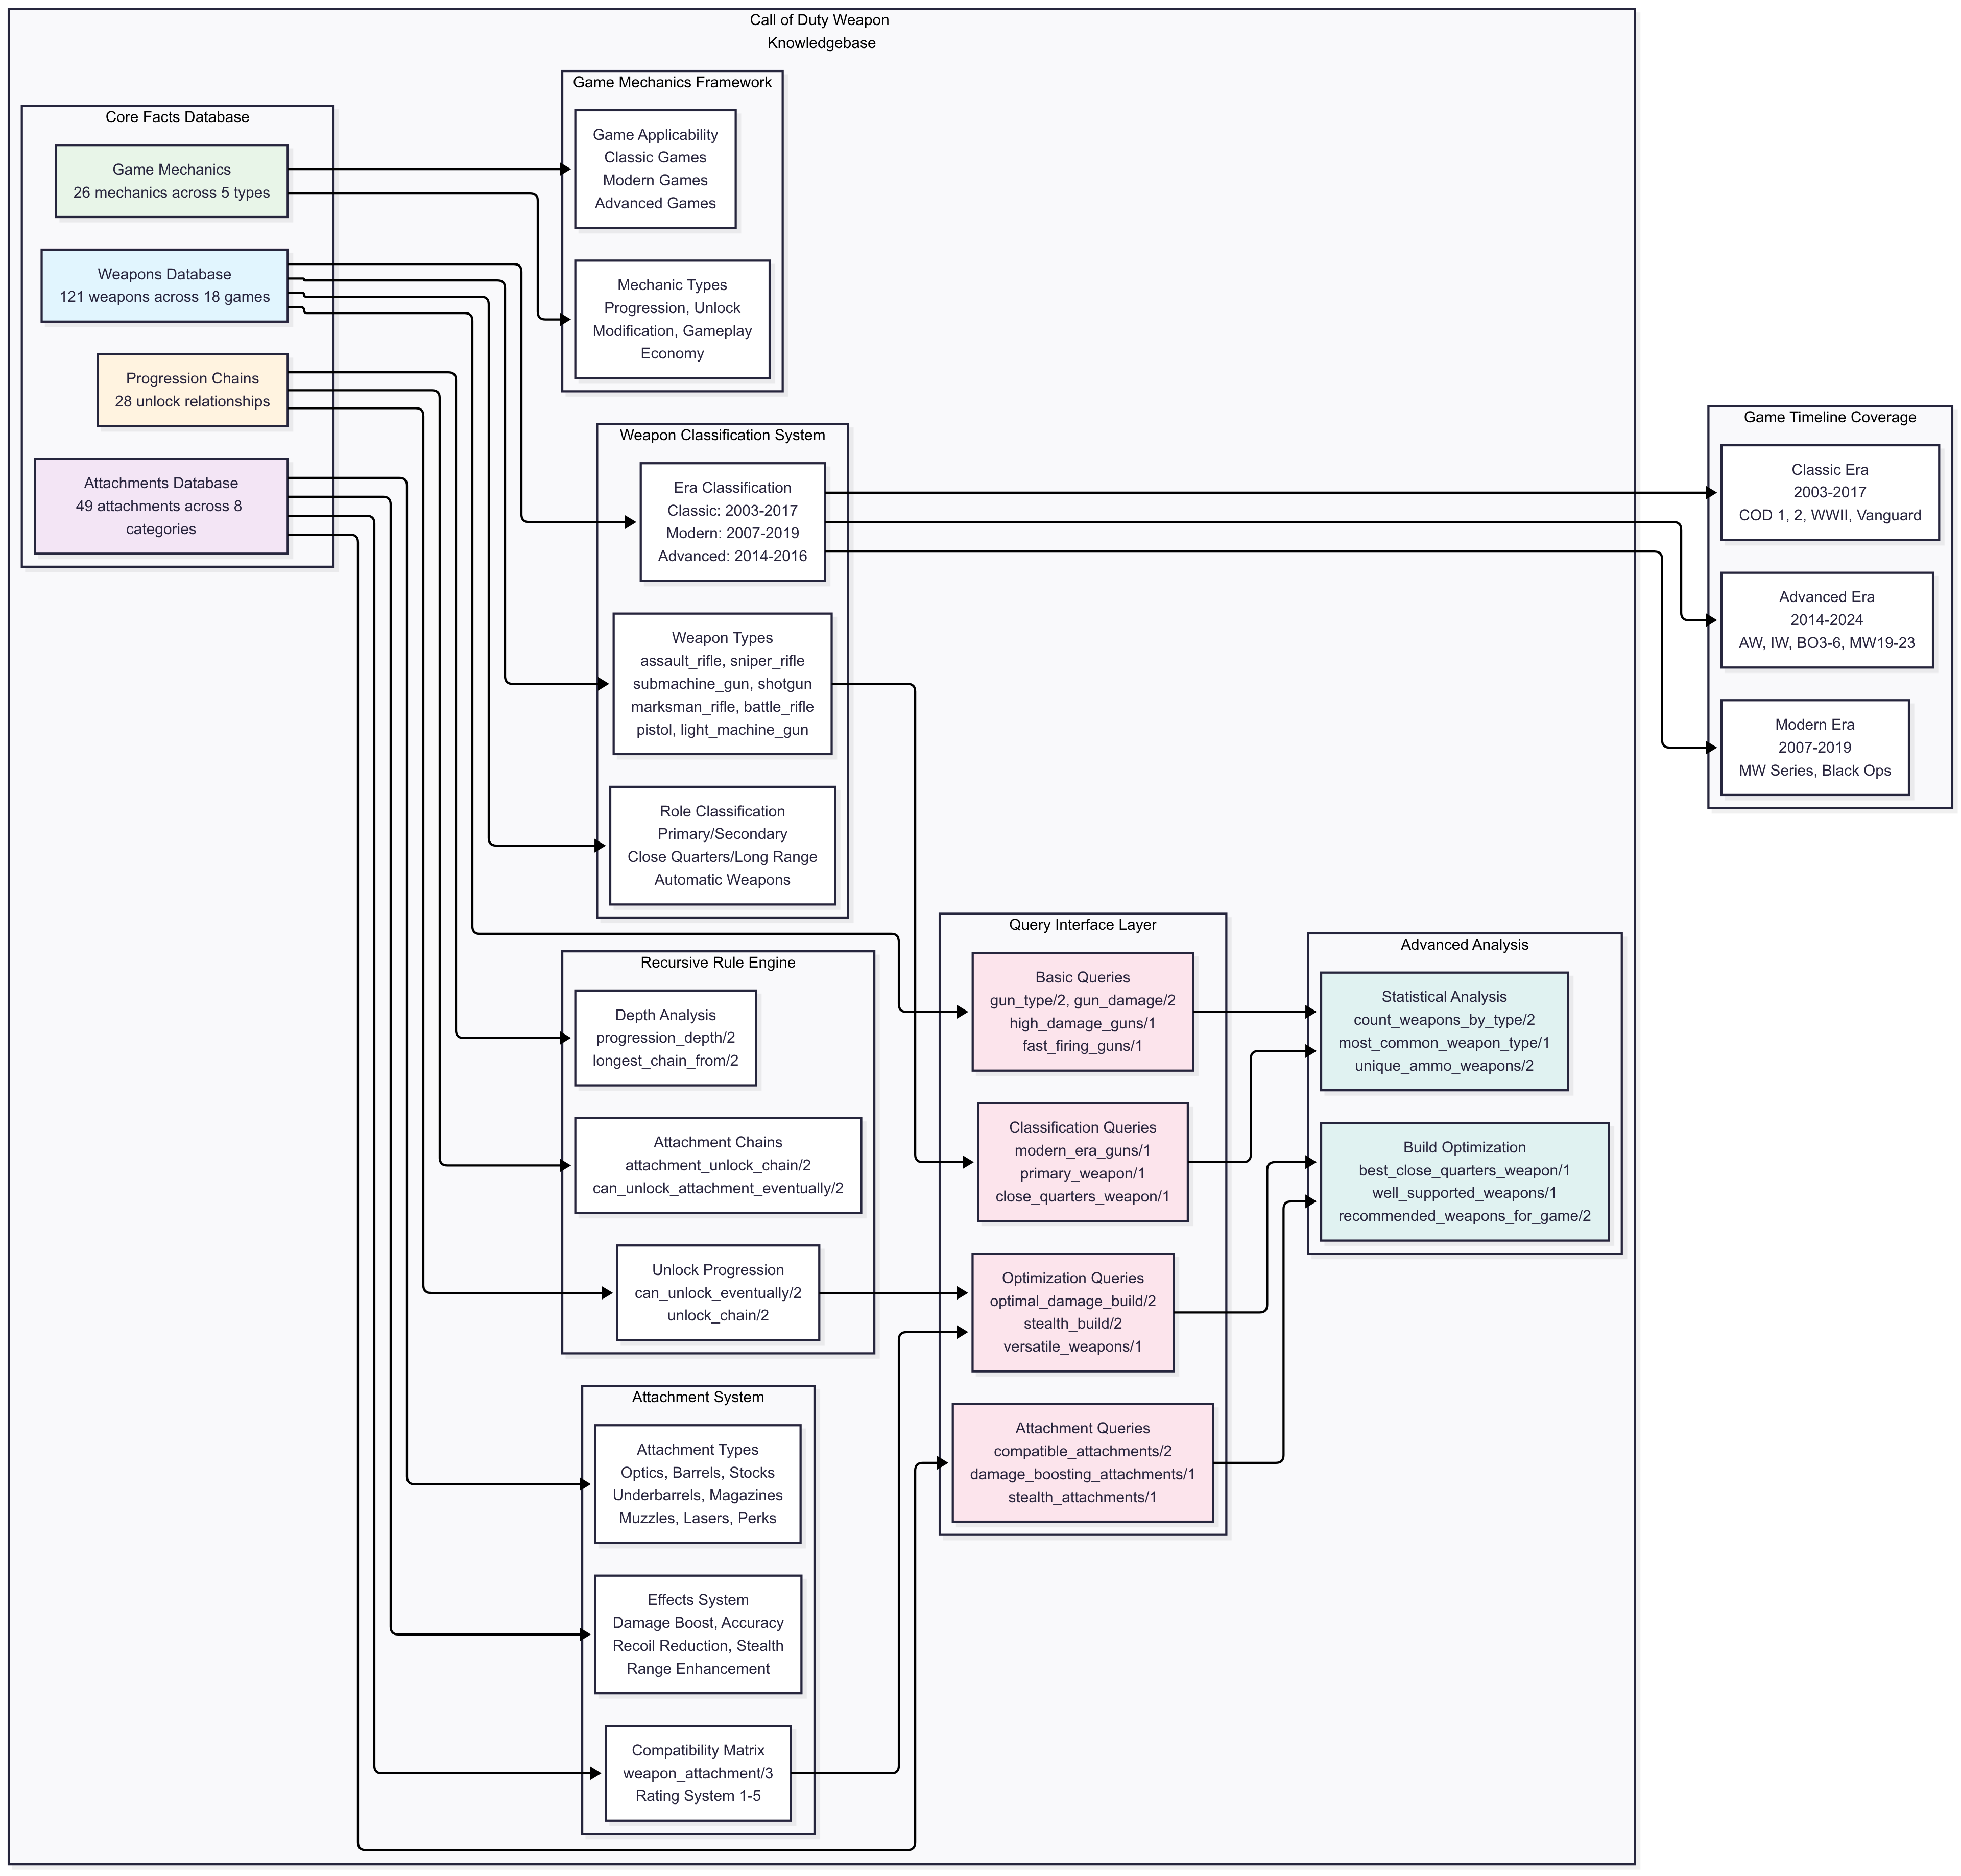
\includegraphics[width=0.8\textwidth]{../diagrams/knowledgebase-diagram-vertical.png}
    \caption{Call of Duty Weapon Knowledgebase System Architecture}
\end{figure}

\subsection{System Architecture Components}

The knowledgebase was designed following a simple-yet-powerful architecture,
reflecting the way I actually think about weapons while gaming. At its heart
lies a complete database of 121 weapons with stats, 49 attachments, and 26 game
mechanics, but the real beauty lies in how these are interrelated. For
instance, the system is capable of dealing with the fact that an M4A1 falls
simultaneously into the category of assault rifle and modern-era weapon, while
also being a general purpose weapon adaptable to a number of different
playstyles. What I cherish most in my system is the recursive engine that can
trace complex paths of unlocks like M4A1 → ACR → MK14, and the recommendation
system that uses various criteria and suggests builds from stealth, damage, and
accuracy. Instead of forcing the user to create complicated Prolog queries, I
created more than 30 predicates that answer natural questions gamers ask, like
"What's the fastest way to unlock the XM4?" or "Which attachments make this gun
better for close-quarters combat?" It's like having a gaming friend who pros
the knowledge of every weapon stat and unlock path in two decades' worth of
Call of Duty titles.

\subsection{Weapon Classification Hierarchy}

The weapon classification system is organized in a hierarchical structure that
categorizes weapons by type, family relationships, and evolutionary
progression, as shown in Figure 2.

\begin{figure}[H]
    \centering
    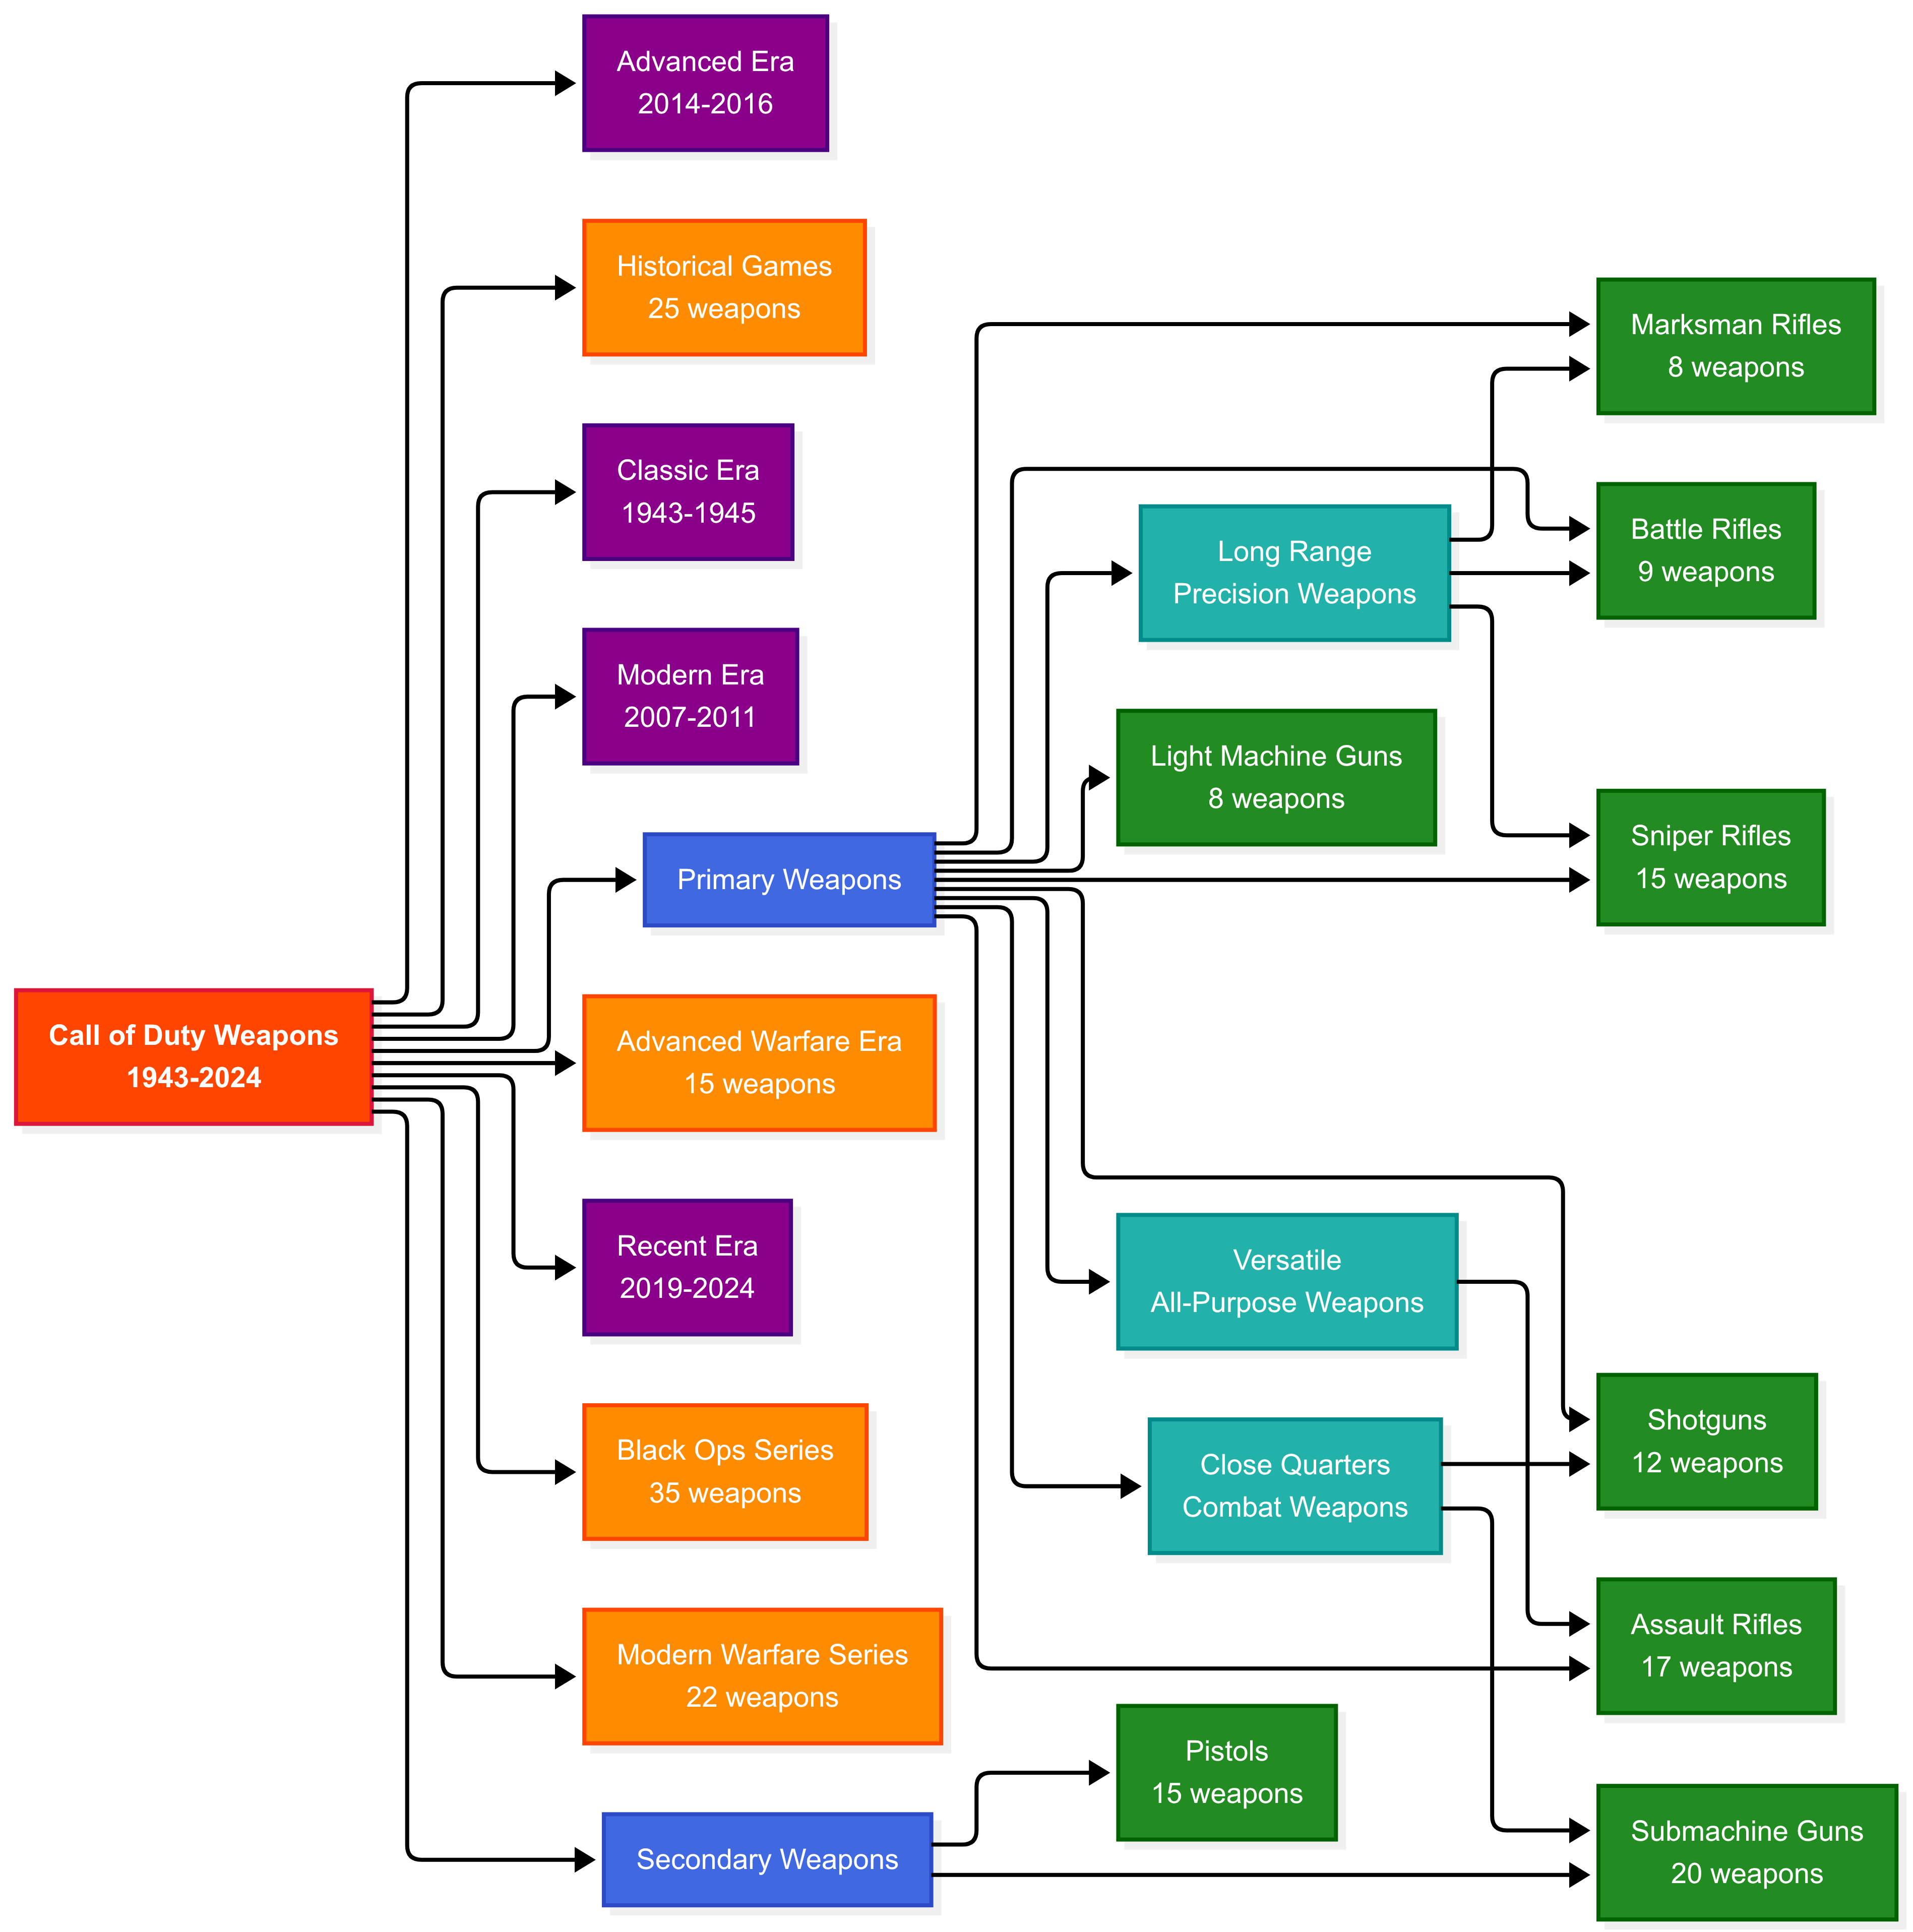
\includegraphics[width=0.9\textwidth]{../diagrams/weapon-type-family-classification-vertical.png}
    \caption{Weapon Type Family Classification Structure}
\end{figure}

\subsection{Weapon Progression System}

The progression system implements complex unlock chains where weapons are
interconnected through prerequisite relationships, enabling recursive analysis
of progression paths as demonstrated in Figure 3.

\begin{figure}[H]
    \centering
    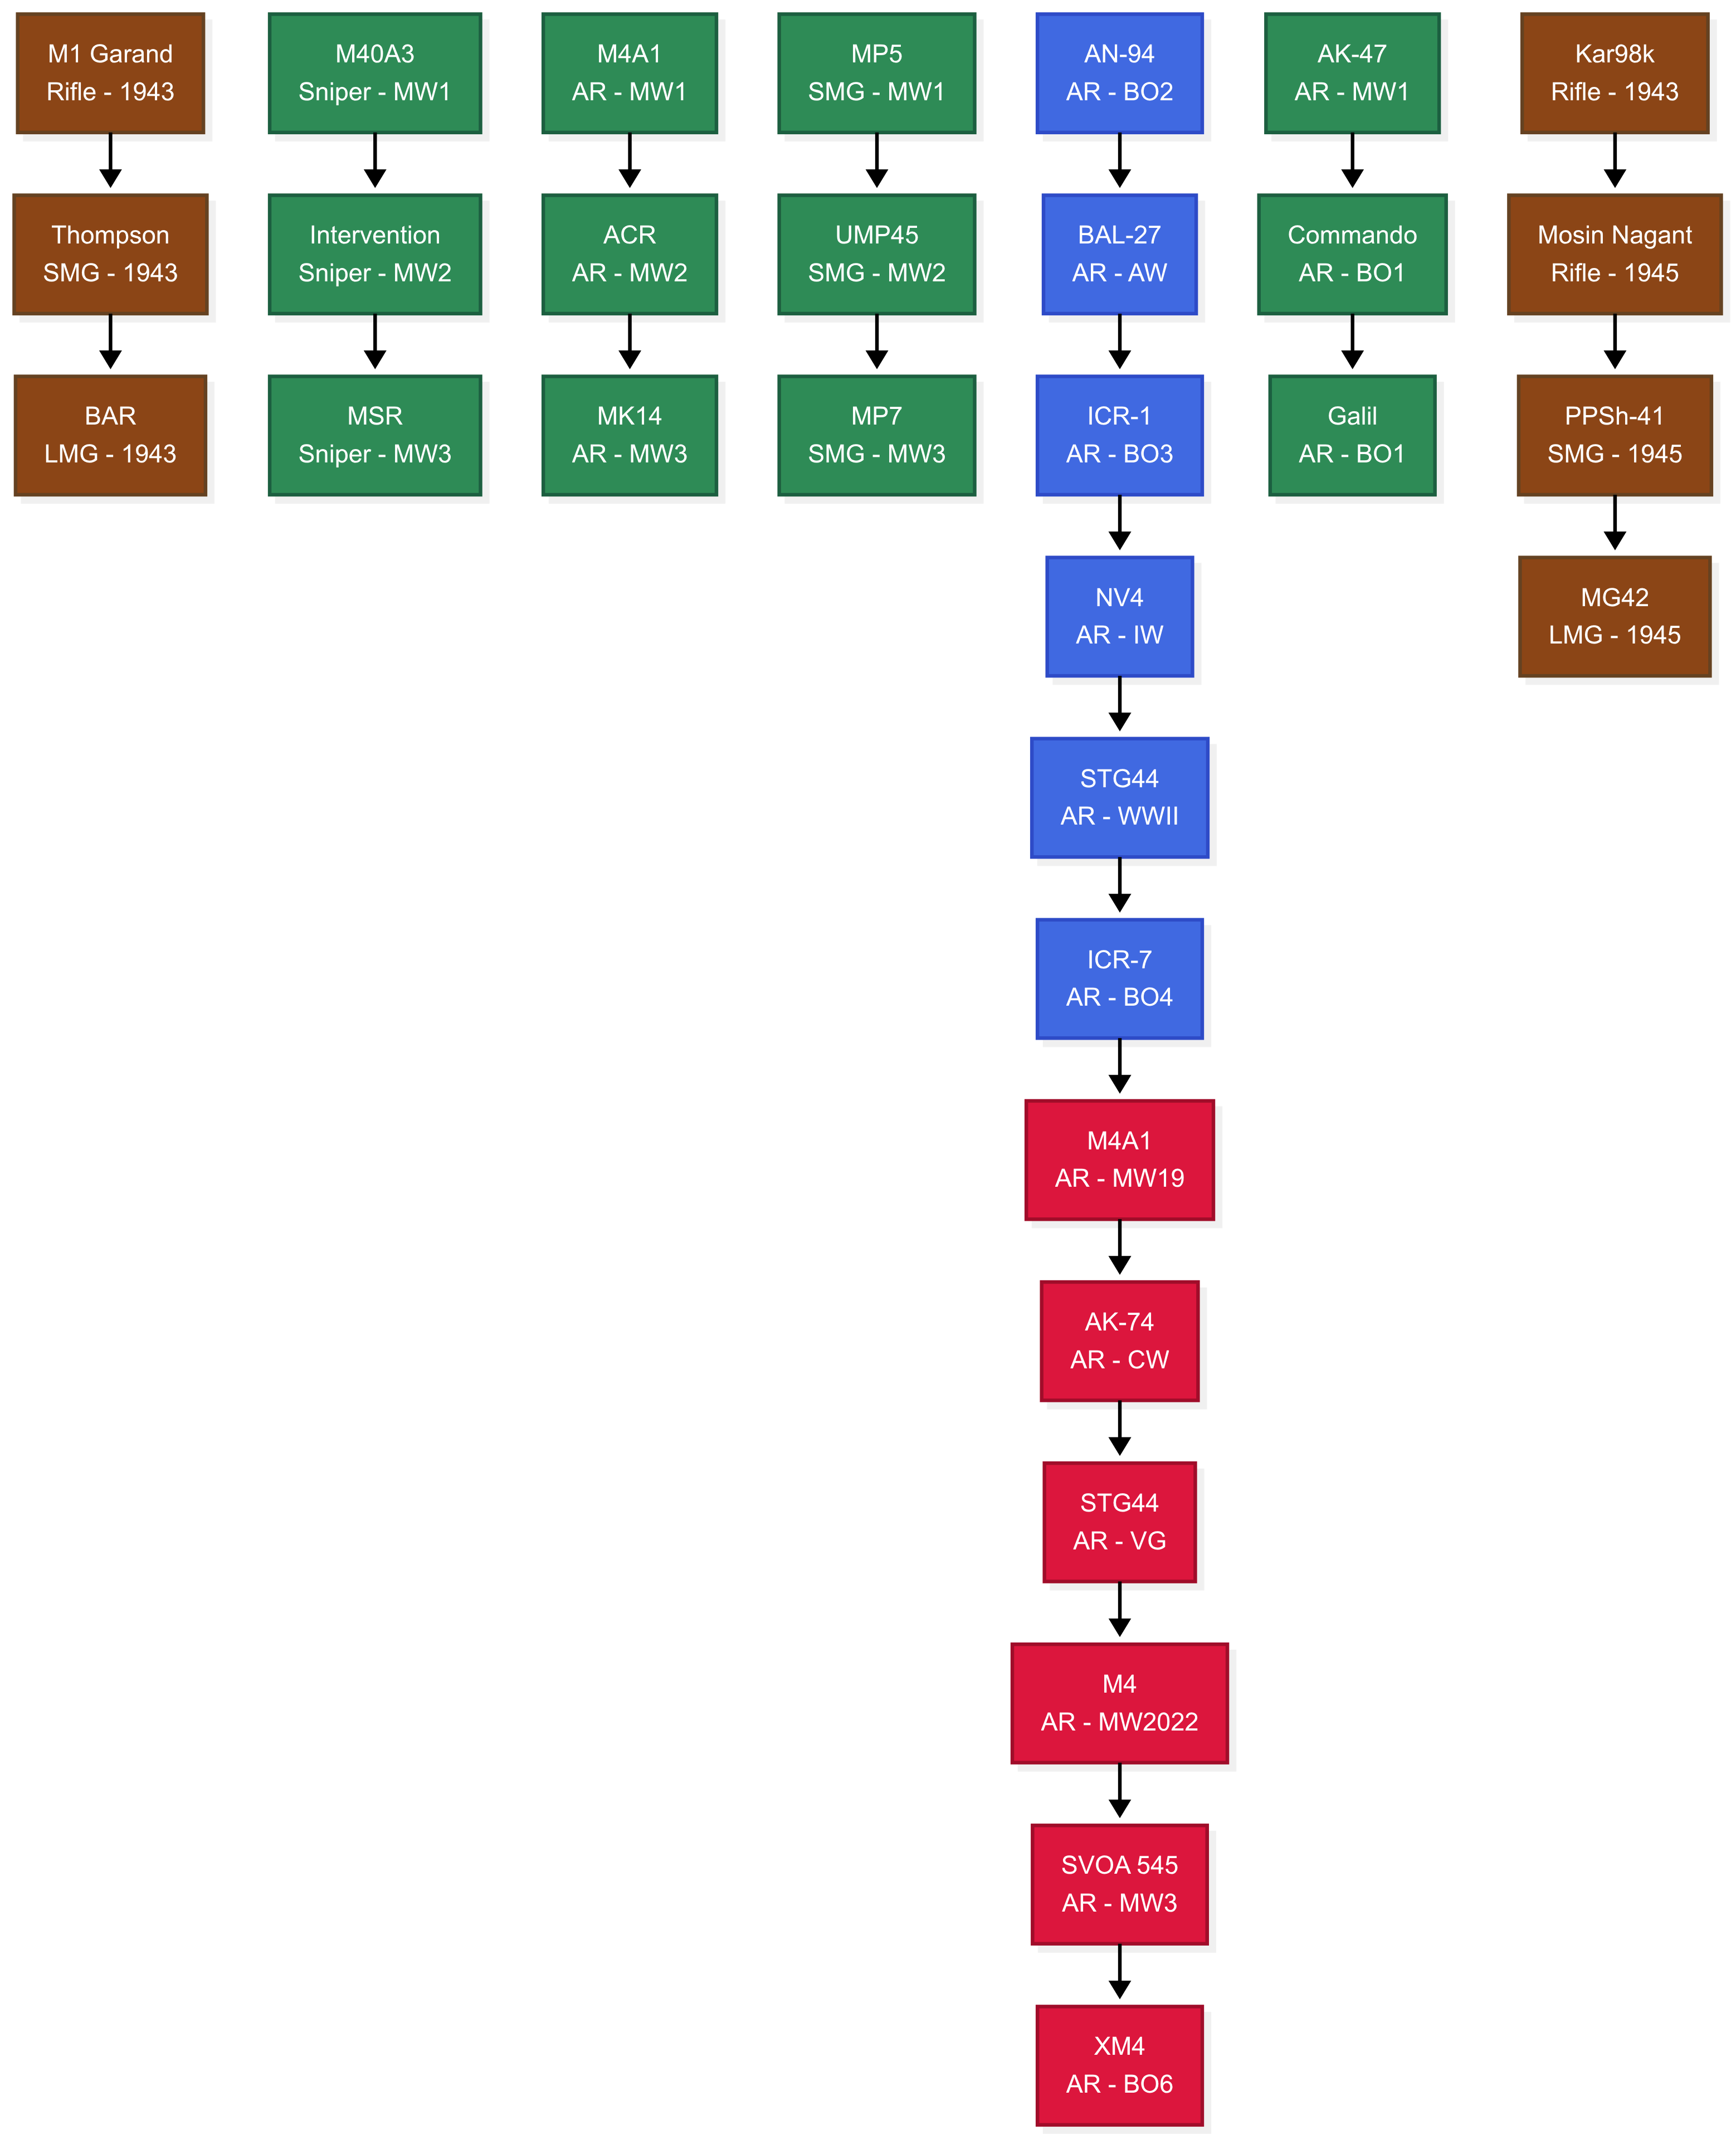
\includegraphics[width=0.9\textwidth]{../diagrams/weapon-progression-family-tree-vertical.png}
    \caption{Weapon Progression Family Tree and Unlock Chains}
\end{figure}

\subsection{Attachment Progression Framework}

The attachment system features its own progression hierarchy where advanced
attachments require unlocking prerequisite attachments, creating complex
dependency chains illustrated in Figure 4.

\begin{figure}[H]
    \centering
    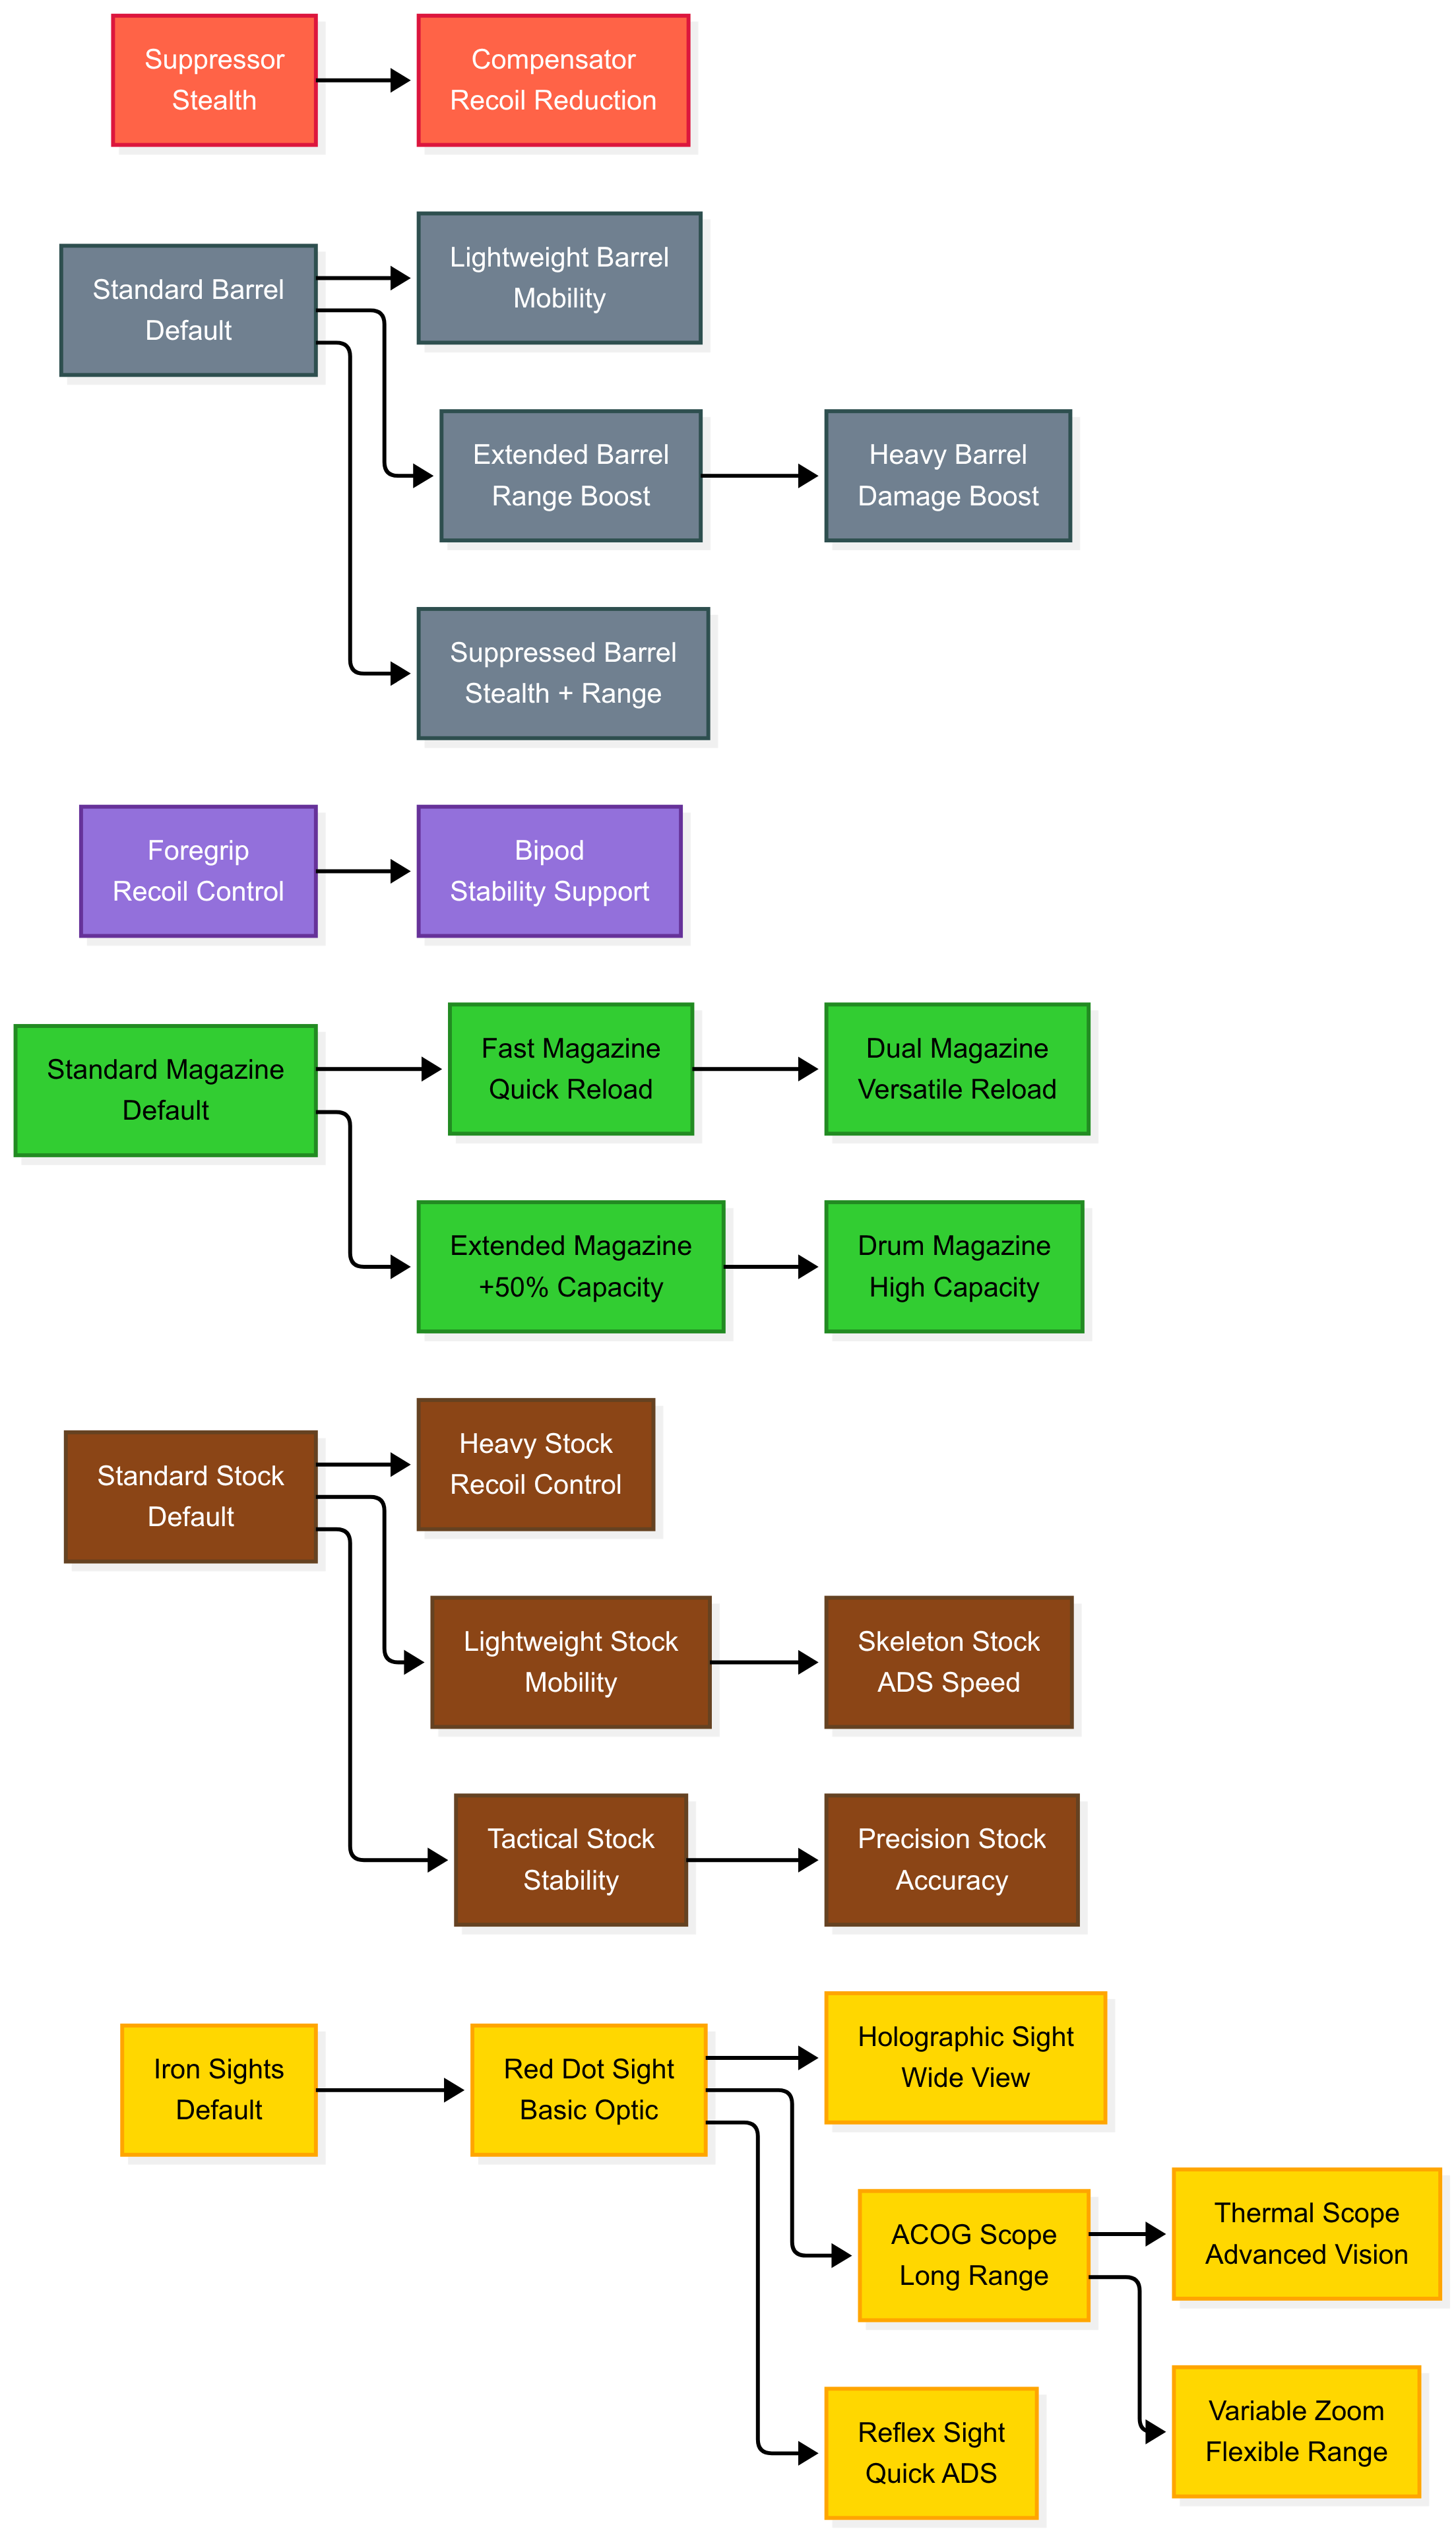
\includegraphics[width=0.9\textwidth]{../diagrams/attachment-progression-family-tree-vertical.png}
    \caption{Attachment Progression Family Tree and Dependencies}
\end{figure}

\subsection{Game Mechanics Evolution}

The evolution of game mechanics across different Call of Duty titles shows the
progression of complexity and feature development over the franchise's history,
as visualized in Figure 5.

\begin{figure}[H]
    \centering
    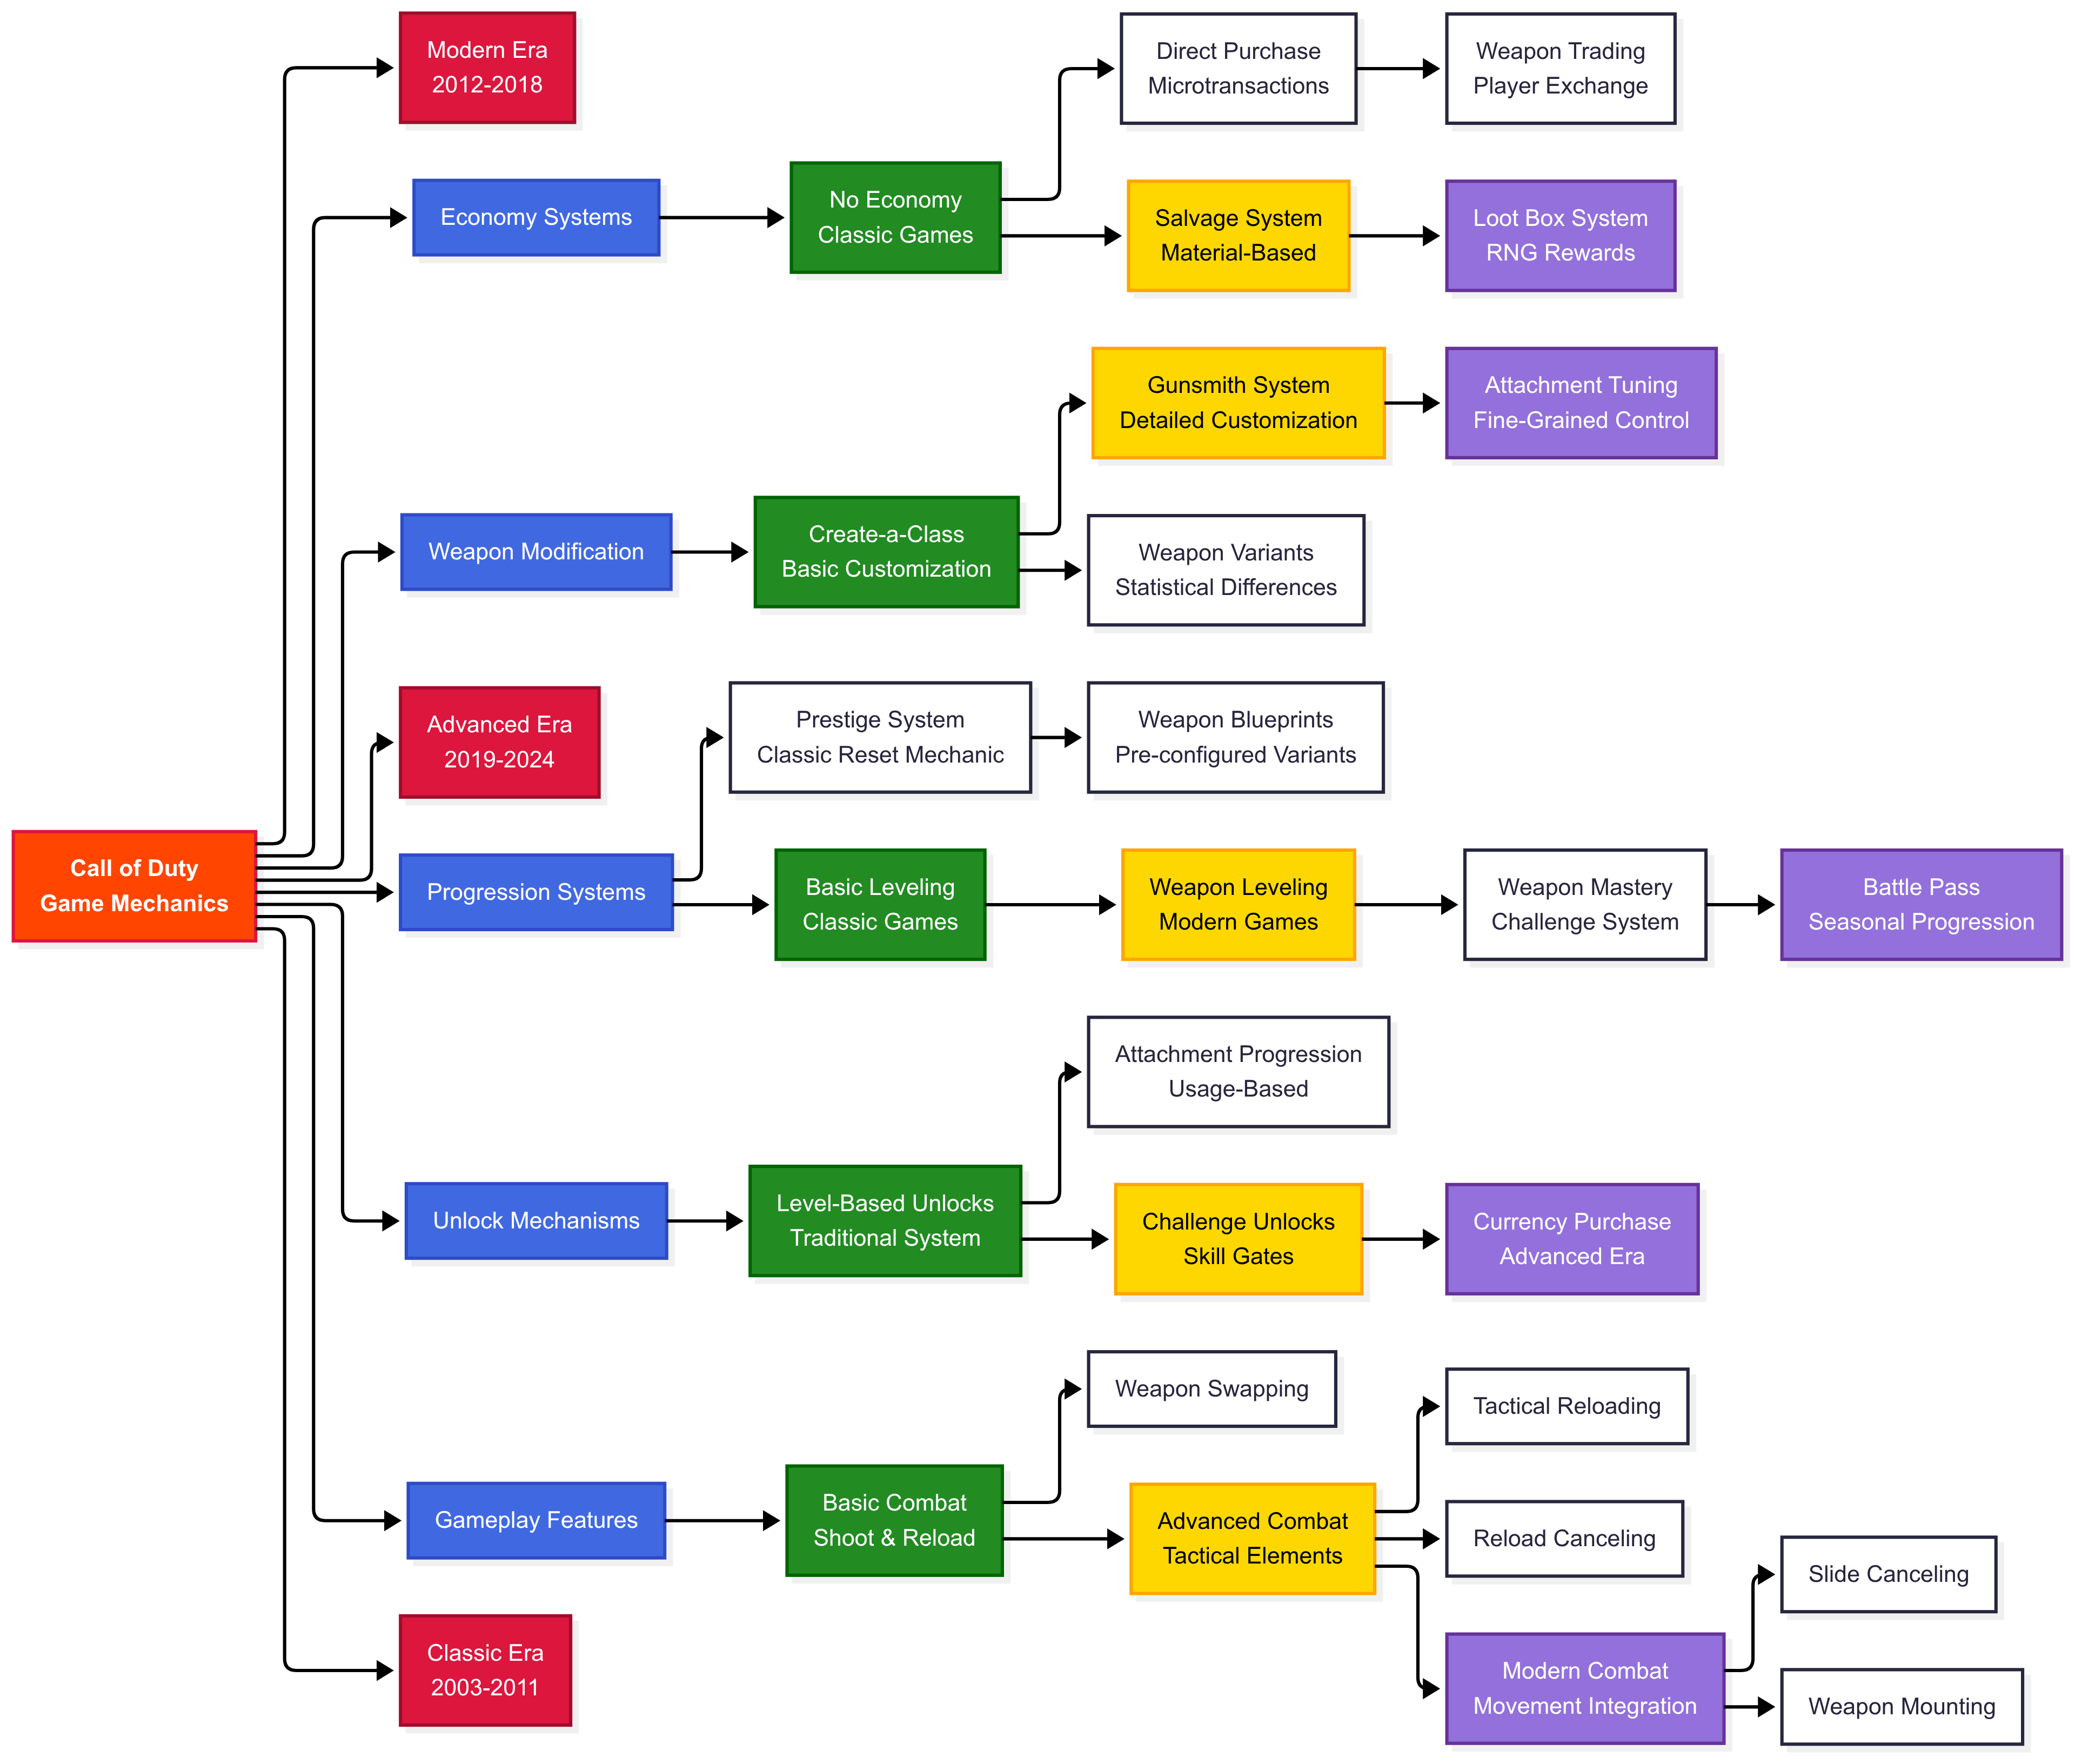
\includegraphics[width=0.9\textwidth]{../diagrams/game-mechanics-evolution-tree-vertical.png}
    \caption{Game Mechanics Evolution Across Call of Duty Titles}
\end{figure}

\section{Sample Input/Output}

\subsection{Basic Weapon Queries}

\textbf{Query}: Find all assault rifles in the knowledgebase
\begin{lstlisting}[language=Prolog]
?- gun_type(assault_rifle, Gun).
\end{lstlisting}

\textbf{Output}:
\begin{lstlisting}
Gun = m4a1 ;
Gun = ak47 ;
Gun = acr ;
Gun = commando ;
Gun = galil ;
Gun = an94 ;
Gun = bal27 ;
Gun = icr1 ;
Gun = nv4 ;
Gun = stg44 ;
Gun = icr7 ;
Gun = m4a1_mw19 ;
Gun = ak74 ;
Gun = stg44_vg ;
Gun = m4_mw2 ;
Gun = svoa_545 ;
Gun = xm4.
\end{lstlisting}

\subsection{Advanced Recursive Queries}

\textbf{Query}: Check if M4A1 can eventually unlock XM4 through progression
\begin{lstlisting}[language=Prolog]
?- can_unlock_eventually(m4a1, xm4).
\end{lstlisting}

\textbf{Output}:
\begin{lstlisting}
true.
\end{lstlisting}

\textbf{Query}: Get the complete unlock chain starting from M4A1
\begin{lstlisting}[language=Prolog]
?- unlock_chain(m4a1, Chain).
\end{lstlisting}

\textbf{Output}:
\begin{lstlisting}
Chain = [m4a1, acr, mk14].
\end{lstlisting}

\subsection{Complex Analysis Queries}

\textbf{Query}: Find weapons suitable for stealth builds
\begin{lstlisting}[language=Prolog]
?- stealth_build(Gun, Attachments),
   length(Attachments, Count),
   Count > 0.
\end{lstlisting}

\textbf{Output}:
\begin{lstlisting}
Gun = m4a1,
Attachments = [suppressor],
Count = 1 ;

Gun = mp5,
Attachments = [suppressor],
Count = 1 ;

Gun = m40a3,
Attachments = [suppressor],
Count = 1.
\end{lstlisting}

\textbf{Query}: Calculate progression depth for XM4
\begin{lstlisting}[language=Prolog]
?- progression_depth(xm4, Depth).
\end{lstlisting}

\textbf{Output}:
\begin{lstlisting}
Depth = 6.
\end{lstlisting}

\subsection{Statistical Analysis}

\textbf{Query}: Find the most common weapon type
\begin{lstlisting}[language=Prolog]
?- most_common_weapon_type(Type).
\end{lstlisting}

\textbf{Output}:
\begin{lstlisting}
Type = assault_rifle.
\end{lstlisting}

\textbf{Query}: Count weapons by type
\begin{lstlisting}[language=Prolog]
?- count_weapons_by_type(assault_rifle, Count).
\end{lstlisting}

\textbf{Output}:
\begin{lstlisting}
Count = 17.
\end{lstlisting}

\subsection{Optimization Queries}

\textbf{Query}: Find optimal damage build for AK-47
\begin{lstlisting}[language=Prolog]
?- optimal_damage_build(ak47, Attachments).
\end{lstlisting}

\textbf{Output}:
\begin{lstlisting}
Attachments = [heavy_barrel, compensator].
\end{lstlisting}

\subsection{Era-Based Classification Queries}

\textbf{Query}: Find all weapons from the modern era
\begin{lstlisting}[language=Prolog]
?- modern_era_guns(Gun).
\end{lstlisting}

\textbf{Output}:
\begin{lstlisting}
Gun = m4a1 ;
Gun = ak47 ;
Gun = mp5 ;
Gun = m249_saw ;
Gun = m40a3 ;
Gun = desert_eagle ;
Gun = w1200 ;
Gun = acr ;
Gun = intervention.
\end{lstlisting}

\subsection{Attachment Compatibility Queries}

\textbf{Query}: Find highly compatible attachments for MP5
\begin{lstlisting}[language=Prolog]
?- highly_compatible_attachments(mp5, Attachment).
\end{lstlisting}

\textbf{Output}:
\begin{lstlisting}
Attachment = suppressor ;
Attachment = extended_mag ;
Attachment = laser_sight.
\end{lstlisting}

\subsection{Weapon Performance Analysis}

\textbf{Query}: Find weapons suitable for close quarters combat
\begin{lstlisting}[language=Prolog]
?- best_close_quarters_weapon(Gun).
\end{lstlisting}

\textbf{Output}:
\begin{lstlisting}
Gun = ppsh_41 ;
Gun = mp5 ;
Gun = ump45 ;
Gun = mp7.
\end{lstlisting}

\textbf{Query}: Find well-supported weapons (3+ attachments)
\begin{lstlisting}[language=Prolog]
?- well_supported_weapons(Gun).
\end{lstlisting}

\textbf{Output}:
\begin{lstlisting}
Gun = m4a1 ;
Gun = ak47 ;
Gun = mp5 ;
Gun = intervention ;
Gun = m249_saw.
\end{lstlisting}

\subsection{Game Mechanics Queries}

\textbf{Query}: Find progression-related game mechanics
\begin{lstlisting}[language=Prolog]
?- progression_mechanics(Mechanic).
\end{lstlisting}

\textbf{Output}:
\begin{lstlisting}
Mechanic = weapon_leveling ;
Mechanic = prestige_system ;
Mechanic = weapon_mastery ;
Mechanic = battle_pass ;
Mechanic = weapon_blueprints ;
Mechanic = camo_challenges.
\end{lstlisting}

\section{Conclusion}

Building this Call of Duty weapon knowledge base has been one funky journey
that surpassed my expectations. Initially, the idea had been to simply present
data about weapons, but over time, that simple premise grew into a complex
system harboring 121 weapons, 49 attachments, and 30+ smart queries that can
now answer questions I've entertained while gaming! The recursive unlocking
system was just the crowning glory-Made prolog trace unlock paths like M4A1 →
ACR → MK14 in one glare of an eye-like magic. I did get into real problems with
performance tuning, attachment compatibility rating, full-fledged testing, and
all sorts of things, but every single problem that popped up was a
very-nice-teacher-allied-with-me lesson-on-prolog-to-ensure-productivity. The
project so much enhanced my outlook over logic programming to merely an
academic curiosity into an efficacious tool for modeling very complicated
relationships. The biggest surprise came with the knowledge that this
knowledgebase is actually practical for gaming support; I have used it for
planning unlock strategies and build recommendations that genuinely help my
gameplay. It is a testament that when passion for a subject is coupled with the
right programming tools, something bridging academic

\end{document}
